\subsection{Ebike Specification} % Main appendix title

\label{appendix:ebike_spec} % For referencing this appendix elsewhere, use \ref{appendixA}

\rhead{Appendix \ref{appendix:ebike_spec}. \emph{Specification of the test ebike}} % This is for the header on each page - perhaps a shortened title

Table \ref{tab:ebike_spec} details the specification of the ebike provided for use over the course of the project.

\begin{table}[H]
\centering
\caption{Ebike Specification}
\label{tab:ebike_spec}
\begin{tabular}{|P{0.3\textwidth}|P{0.3\textwidth}|}
\hline
\multicolumn{2}{|l|}{\textbf{Ebike}}     \\
\hline
\hline
Model           & Unknown     \\
\hline
Wheel diameter  & 311mm       \\
\hline
Weight          & 15kg        \\
\hline
\hline
\multicolumn{2}{|l|}{\textbf{Battery}}   \\
\hline
\hline
Type            & Lithium Ion \\
\hline
Capacity        & 6Ah         \\
\hline
Rated voltage   & 36V         \\
\hline
\hline
\multicolumn{2}{|l|}{\textbf{Motor}}     \\
\hline
\hline
Type            & Brushless   \\
\hline
Rated power     & 250W        \\
\hline
Rated voltage   & 36V         \\
\hline
Rated RPM       & 78rpm       \\
\hline
Rated torque    & 30Nm        \\
\hline
\hline
\multicolumn{2}{|l|}{\textbf{Display Monitor}} \\
\hline
\hline
Type            & LCD S900 \\  
\hline
\end{tabular}
\end{table}

Figure \ref{fig:motor_characteristic_curve} illustrates the ebike motor's characteristic curves.

\begin{figure}[H]
    \centering
    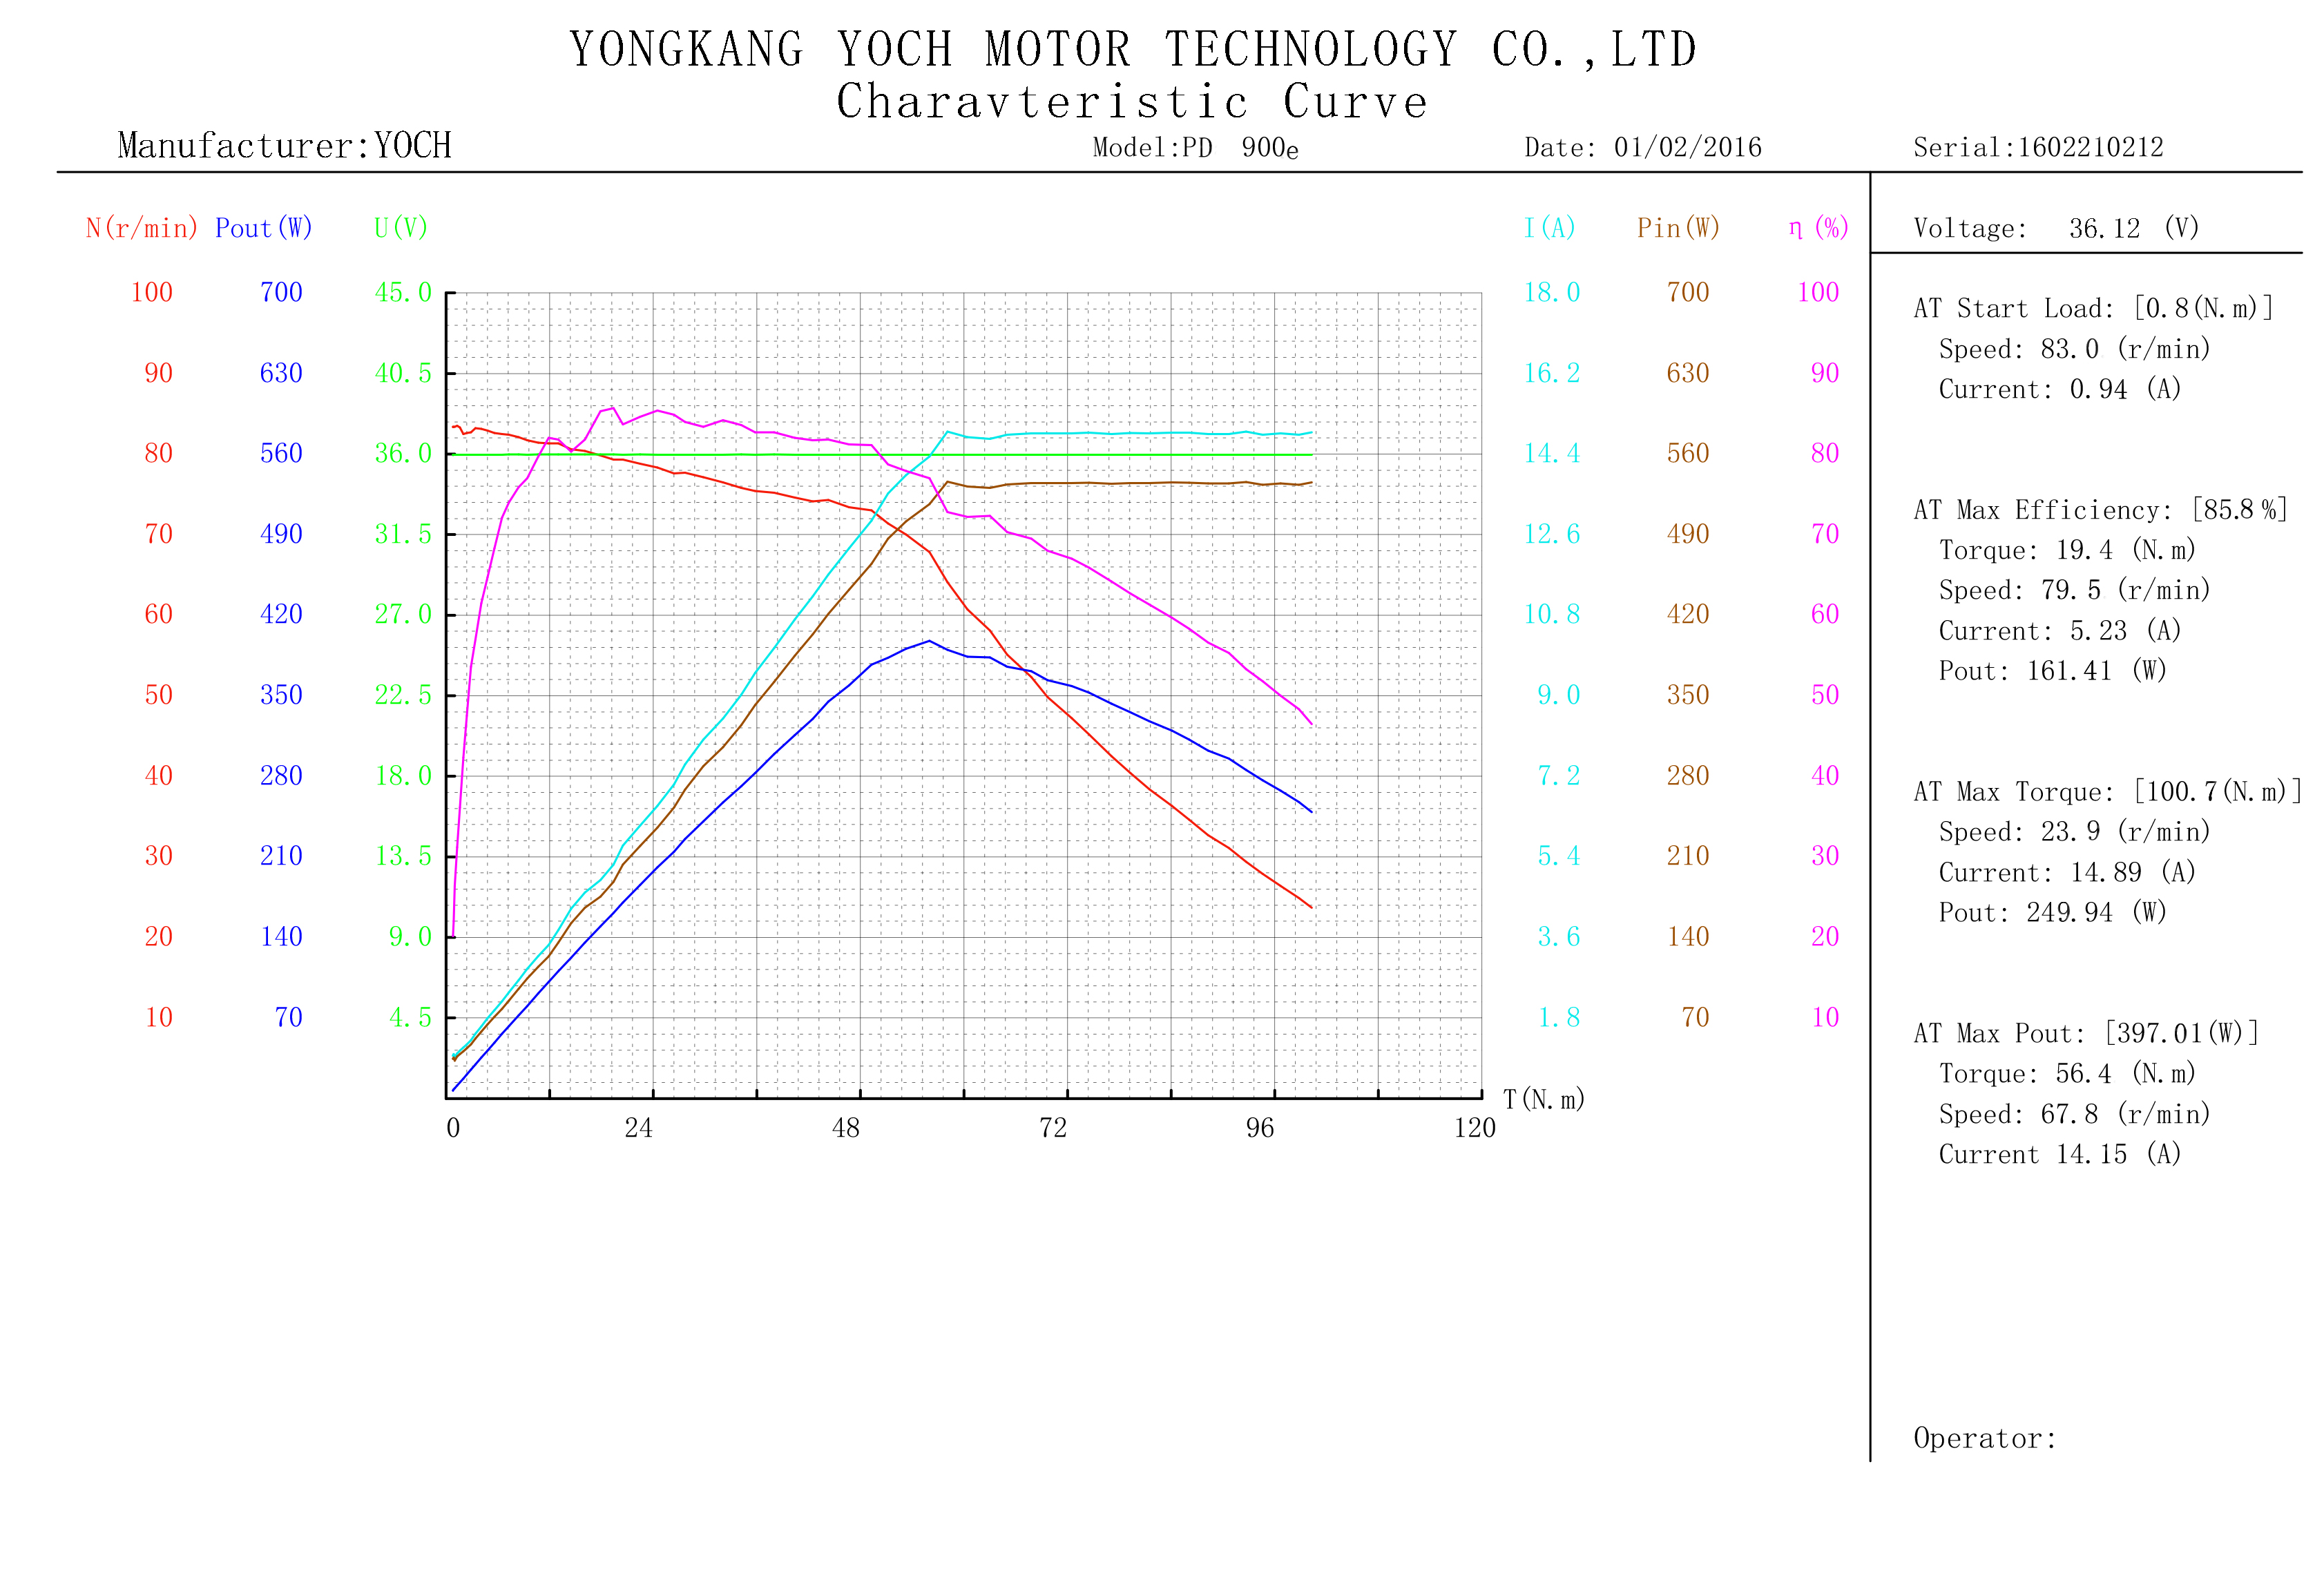
\includegraphics[width=\textwidth]{images/Motor_Characteristic_Curve.jpg}
    \caption{Motor Characteristic Curve}
    \label{fig:motor_characteristic_curve}
\end{figure}